\begin{question}
\noindent Triangle $T$ has vertices at $A(1,2)$, $B(3,2)$ and $C(1,4)$.

\noindent Find the coordinates of the image of triangle $T$ after a reflection in the line $y=1$.

\begin{center}
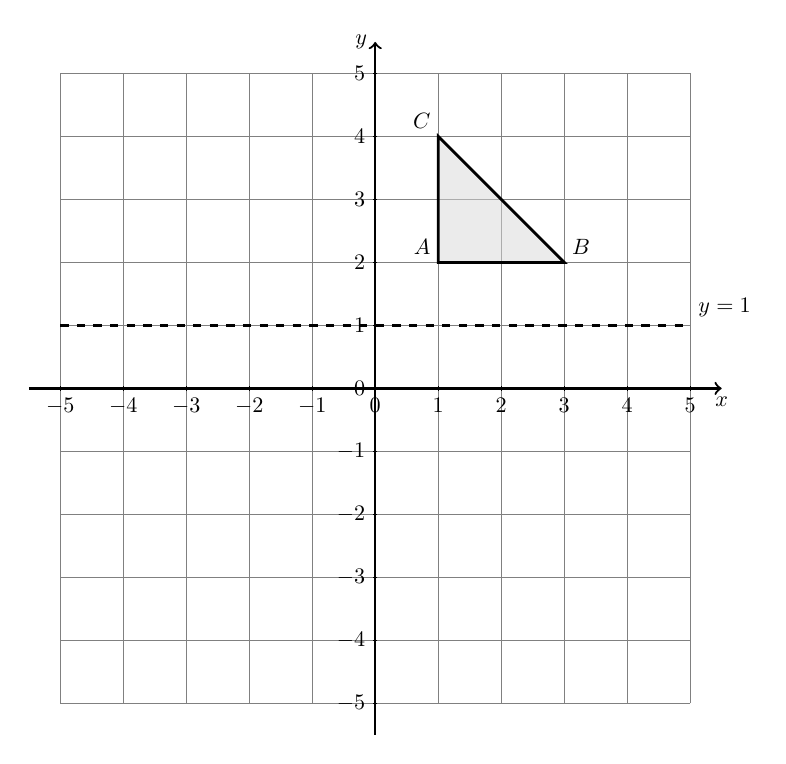
\begin{tikzpicture}[scale=0.8, transform shape]
    % Define colours
    \definecolor{borderColour}{HTML}{000000}
    \definecolor{fillColour}{HTML}{D8D8D8}

    % Define axis scale
    \def\axisLimit{5}

    % Draw grid
    \draw[step=1cm,gray,very thin] (-\axisLimit,-\axisLimit) grid (\axisLimit,\axisLimit);

    % Draw axes
    \draw[thick,->] (-\axisLimit-0.5,0) -- (\axisLimit+0.5,0) node[anchor=north] {$x$};
    \draw[thick,->] (0,-\axisLimit-0.5) -- (0,\axisLimit+0.5) node[anchor=east] {$y$};

    % Label x-axis and y-axis
    \foreach \x in {-\axisLimit,...,\axisLimit}
        \draw (\x cm,1pt) -- (\x cm,-1pt) node[anchor=north] {$\x$};
    \foreach \y in {-\axisLimit,...,\axisLimit}
        \draw (1pt,\y cm) -- (-1pt,\y cm) node[anchor=east] {$\y$};

    % Draw the reflection line y = 1
    \draw[thick,dashed] (-5,1) -- (5,1) node[anchor=south west] {$y=1$};

    % Define coordinates for the vertices of triangle T
    \coordinate (A) at (1,2);
    \coordinate (B) at (3,2);
    \coordinate (C) at (1,4);

    % Draw triangle T
    \filldraw[fill=fillColour, draw=borderColour, line width=1pt, fill opacity=0.5] (A) -- (B) -- (C) -- cycle;

    % Label the vertices of triangle T
    \node[above left] at (A) {$A$};
    \node[above right] at (B) {$B$};
    \node[above left] at (C) {$C$};

\end{tikzpicture}
\end{center}

\vspace{4cm}
\begin{flushright}
    \answerplain{2}
\end{flushright}
\end{question}
